\documentclass[titlepage, fleqn, a4paper, 12pt, twoside]{article}
\usepackage{geometry}
\usepackage{exsheets} %question and solution environments
\usepackage{amsmath, amssymb, amsthm} %standard AMS packages
\usepackage[utf8]{inputenc}
\usepackage{esint} %integral signs
\usepackage{marginnote} %marginnotes
\usepackage{gensymb} %miscellaneous symbols
\usepackage{commath} %differential symbols
\usepackage{xcolor} %colours
\usepackage{cancel} %cancelling terms
\usepackage[free-standing-units,space-before-unit]{siunitx} %formatting units
	\sisetup
	{
		per-mode=fraction,
		fraction-function=\frac
	}
\usepackage{tikz, pgfplots} %diagrams
	\usetikzlibrary{calc, hobby, patterns, intersections, angles, quotes, spy}
\usepackage{graphicx} %inserting graphics
\usepackage{hyperref} %hyperlinks
\usepackage{datetime} %date and time
\usepackage{enumerate, enumitem} %numbered lists
\usepackage{float} %inserting floats
\usepackage[american voltages]{circuitikz} %circuit diagrams
\usepackage{setspace} %double spacing
\usepackage{microtype} %micro-typography
\usepackage{listings} %formatting code
	\lstset{language=Matlab}
	\lstdefinestyle{standardMatlab}
	{
		belowcaptionskip=1\baselineskip,
		breaklines=true,
		frame=L,
		xleftmargin=\parindent,
		language=C,
		showstringspaces=false,
		basicstyle=\footnotesize\ttfamily,
		keywordstyle=\bfseries\color{green!40!black},
		commentstyle=\itshape\color{purple!40!black},
		identifierstyle=\color{blue},
		stringstyle=\color{orange},
	}
\usepackage{algpseudocode} %algorithms
\usepackage{algorithm} %algorithms
\usepackage{chemfig}
\usepackage{booktabs}
\usepackage{multirow}
\usepackage{todonotes}
\usepackage[noabbrev,capitalize]{cleveref}

\newcommand\numberthis{\addtocounter{equation}{1}\tag{\theequation}} %adds numbers to specific equations in non-numbered list of equations

\theoremstyle{definition}
\newtheorem{example}{Example}
\newtheorem{definition}{Definition}

\theoremstyle{theorem}
\newtheorem{theorem}{Theorem}
\newtheorem{law}{Law}

\makeatletter
\@addtoreset{section}{part} %resets section numbers in new part
\makeatother

\newcommand\blfootnote[1]{%
	\begingroup
	\renewcommand\thefootnote{}\footnote{#1}%
	\addtocounter{footnote}{-1}%
	\endgroup
}

\renewcommand{\marginfont}{\scriptsize \color{blue}}

\renewcommand{\tilde}{\widetilde}

\SetupExSheets{solution/print = true} %prints all solutions by default

%opening
\title{Electronic Devices}
\author{Aakash Jog}
\date{2015-16}

\begin{document}

\pagenumbering{roman}
\begin{titlepage}
\newgeometry{margin=0cm}
\maketitle
\end{titlepage}
\restoregeometry
%\setlength{\mathindent}{0pt}

\blfootnote
{	
	\begin{figure}[H]
		\includegraphics[height = 12pt]{cc.pdf}
		\includegraphics[height = 12pt]{by.pdf}
		\includegraphics[height = 12pt]{nc.pdf}
		\includegraphics[height = 12pt]{sa.pdf}
	\end{figure}
	This work is licensed under the Creative Commons Attribution-NonCommercial-ShareAlike 4.0 International License. To view a copy of this license, visit \url{http://creativecommons.org/licenses/by-nc-sa/4.0/}.
} %CC-BY-NC-SA license

\tableofcontents

\clearpage
\listoffigures

\clearpage
\section{Lecturer Information}

\textbf{Tammy Ben-Yaacov}\\
~\\
E-mail: \href{mailto:tammybenyaacov@gmail.com}{tammybenyaacov@gmail.com}\\

\section{Instructor Information}

\textbf{Asia Shapira}\\
~\\
E-mail: \href{asiasapi@gmail.com}{asiasapi@gmail.com}

\section{Required Reading}

\begin{enumerate}
	\item Streetman, B. Solid State Electronic Devices
\end{enumerate}

\section{Additional Reading}

\begin{enumerate}
	\item Bar-Lev, A. Semiconductor and Electronic Devices
	\item S. M. Sze, Physics of Semiconductor Devices
	\item Kittel, C. (2005). Introduction to Solid State Physics
\end{enumerate}

\clearpage
\pagenumbering{arabic}

\part{}

\section{Energy Bands in Semiconductors}

\begin{figure}[h]
	\centering
	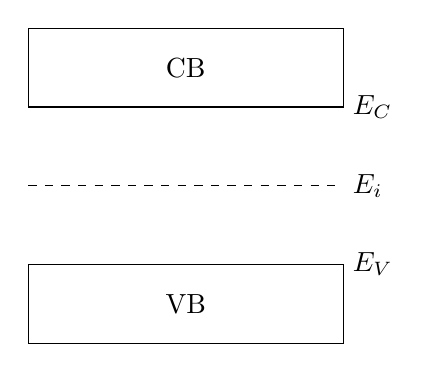
\begin{tikzpicture}
		\def\l{4};
		\def\eConduction{4};
		\def\eValence{2};
		\def\eIntrinsic{{\eConduction * 0.5 + \eValence * 0.5}};

		\begin{scope}
			\draw (0,\eValence) rectangle ++(\l,-1);
			\node at ($ (\l/2,\eValence) + (0,-0.5) $) {VB};
			\node [right] at (\l,\eValence) {$E_V$};
		\end{scope}

		\begin{scope}
			\draw (0,\eConduction) rectangle ++(\l,1);
			\node at ($ (\l/2,\eConduction) + (0,0.5) $) {CB};
			\node [right] at (\l,\eConduction) {$E_C$};
		\end{scope}

		\begin{scope}
			\draw [dashed] (0,\eIntrinsic) -- (\l,\eIntrinsic) node [right] {$E_i$};
		\end{scope}
	\end{tikzpicture}
	\caption{Energy Bands and Intrinsic Energy Level}
	\label{fig:Energy_Bands_and_Intrinsic_Energy_Level}
\end{figure}

\section{Determining Factors for Number of Charge Carriers in Energy Bands}

\subsection{Density of Allowed States in Bands}

The number of allowed states in the conduction and valence bands are denoted as $N_C(E)$ and $N_V(E)$, respectively.\\
There are no allowed states in the gap between the conduction and valence bands.

\begin{theorem}
	\begin{align*}
		N_C(E) & \approx \sqrt{E - E_C}
	\end{align*}
\end{theorem}

\subsection{Probability of Occupancy of Allowed States}

\begin{definition}[Fermi function]
	The probability that an available energy state $E$ will be occupied is
	\begin{align*}
		f(E) & = f_{\text{FD}}(E) \\
                     & = \frac{1}{1 + e^{\frac{E - E_f}{k T}}}
	\end{align*}
	where $E_f$ is the Fermi level or the Fermi energy, and $T$ is the temperature.
\end{definition}
Therefore, the graph of $f(E)$ with respect to $E$ is as in \cref{fig:Graph_of_Fermi_function_for_$T_1_>_T_2_>_T_3$}.
\begin{figure}[h]
	\centering
	\includegraphics[width = 0.8\textwidth]{./Plots/fermi_function.pdf}
	\caption{Graph of Fermi function for $T_1 > T_2 > T_3$}
	\label{fig:Graph_of_Fermi_function_for_$T_1_>_T_2_>_T_3$}
\end{figure}
If $E < E_f$,
\begin{align*}
	\lim\limits_{T \to 0} f(E) & = 1
\end{align*}
If $E = E_f$,
\begin{align*}
	f(E) & = \frac{1}{2}
\end{align*}
If $E_f < E$,
\begin{align*}
	\lim\limits_{T \to 0} f(E) & = 0
\end{align*}
Therefore, at $0 \kelvin$, $f(E)$ is the unit step function.
Therefore, at $0 \kelvin$, all electrons are at available energy levels less than $E_f$, i.e. in the valence band.
Hence, the conduction band is empty.

\section{Number of Electrons in Conduction Band}

\begin{theorem}
	Electrons in semiconductors obey Fermi-Dirac statistics.
\end{theorem}

Consider an energy band of thickness $\dif E$, at energy $E$, in the conduction band.
Therefore, the number of electrons in the band is
\begin{align*}
	\dif n(E) & = N_C(E) f(E) \dif E
\end{align*}
Therefore, the total number of electrons in the conduction band are
\begin{align*}
	n & = \int\limits_{E_C}^{E_{C} + \Delta} N_C(E) f(E) \dif E
\end{align*}
where $\Delta$ is the thickness of the conduction band.\\
As there are no allowed states above the conduction band,
\begin{align*}
	n & = \int\limits_{E_C}^{\infty} N_C(E) f(E) \dif E
\end{align*}

\section{Position of $E_F$}

\subsection{Intrinsic Semiconductor}

In an intrinsic semiconductor,
\begin{equation*}
	n = p = n_i
\end{equation*}
At $0 \kelvin$, all electrons are in the valence band.
Therefore, for all electrons to be below $E_F$, $E_F$ must be between $E_C$ and $E_V$.
Therefore,
\begin{align*}
	E_F & = E_i
\end{align*}
Therefore, the graphs of $f(E)$ and $1 - f(E)$ are as in \cref{fig:Graph_of_$f(E)$_and_$1_-_f(E)$}.
\begin{figure}[h]
	\centering
	\includegraphics[width = 0.8\textwidth]{./Plots/fermi_function_and_one_minus_fermi_function.pdf}
	\caption{Graph of $f(E)$ and $1 - f(E)$}
	\label{fig:Graph_of_$f(E)$_and_$1_-_f(E)$}
\end{figure}

\subsection{N-type Semiconductor}

In a N-type semiconductor,
\begin{align*}
	n & > p
\end{align*}
As $0 \kelvin$, all electrons must be either at in the valence band, or at $E_d$.
Therefore, for all electrons to be below $E_F$, $E_F$ must be between $E_d$ and $E_C$.
Therefore, as $E_d$ is closer to $E_C$ than to $E_V$, $E_F$ is also closer to $E_C$ than to $E_V$.\\
The number of electrons in the conduction band is equal to the area under the curve of $f(E)$, to the right of $E_C$.

\subsection{P-type Semiconductor}

In a P-type semiconductor,
\begin{align*}
	p & > n
\end{align*}
As $0 \kelvin$, all electrons must be either at in the valence band, or at $E_a$.
Therefore, for all electrons to be below $E_F$, $E_F$ must be between $E_a$ and $E_C$.
Therefore, as $E_a$ is closer to $E_V$ than to $E_C$, $E_F$ is also closer to $E_V$ than to $E_C$.

\section{Graphical Representation of Number of Electrons in the Conduction Band}

The number of allowed states in the conduction band is given by
\begin{align*}
	N_C(E) & = \frac{4 \pi}{h^3} \left( 2 {m_e}^* \right)^{\frac{3}{2}} (E - E_C)^{\frac{1}{2}} \\
               & \approx \sqrt{E - E_C}
\end{align*}
The probability of an energy state $E$ being occupied is given by
\begin{align*}
	f(E) & = \frac{1}{1 + e^{\frac{E - E_F}{k T}}}
\end{align*}
Therefore, the electron distribution in the conduction band is
\begin{align*}
	N_C(E) f(E) & = \sqrt{E - E_C} \frac{1}{1 + e^{\frac{E - E_F}{k T}}}
\end{align*}
Therefore, as $N_C(E)$ is zero for $E < E_C$, the graph of the electron distribution function is as in \cref{fig:Electron_distribution_function_in_the_conduction_band}.
\begin{figure}[h]
	\centering
	\includegraphics[width = 0.8\textwidth]{./Plots/electron_distribution_in_conduction_band.pdf}
	\caption{Electron distribution function in the conduction band}
	\label{fig:Electron_distribution_function_in_the_conduction_band}
\end{figure}

\section{Maxwell-Boltzmann Approximation}

The number of allowed states in the gap between the valence and conduction bands is zero.
Therefore, although the Fermi function is non zero in the energy gap, the number of electrons in the conduction band can be approximated as
\begin{align*}
	\frac{1}{1 + e^{\frac{E - E_F}{k T}}} & \approx e^{-\frac{E - E_F}{k T}}
\end{align*}
Therefore, integrating and solving,
\begin{align*}
	n & = N_C e^{\frac{E_C - E_F}{k T}}
\end{align*}
where $N_C$ is a constant which represents the effective density of states, and not a function of $E$.\\
Therefore, at equilibrium,
\begin{align*}
	n_0 & = N_C e^{-\frac{E_C - E_F}{k T}} \\
	p_0 & = N_V e^{-\frac{E_F - E_V}{k T}}
\end{align*}
Therefore,
\begin{align*}
	{n_i}^2        & = n_0 p_0                            \\
                       & = N_C N_V e^{-\frac{E_C - E_V}{k T}} \\
	\therefore n_i & = \sqrt{N_C N_V} e^{-\frac{E_{\text{gap}}}{k T}}
\end{align*}

\end{document}
